% Original book diagram: fig:robotic_digital_twin_workflow_DT
% Book source: sections/Part_V/DT.tex
% Original diagram authorship retained. Visual design: Ziad Mosalam.
\documentclass[11pt,border=8pt]{standalone}
\usepackage{amsmath,amssymb,graphicx,tikz}
\usetikzlibrary{arrows.meta,automata,positioning,calc,shapes.geometric,fit,backgrounds,patterns}
\newcommand{\vect}[1]{\mathbf{#1}}
\newcommand{\mat}[1]{\mathbf{#1}}
\newcommand{\Normal}{\mathcal{N}}
\newcommand{\prob}{p}
\newcommand{\E}{\mathbb{E}}
\newcommand{\Var}{\mathrm{Var}}
\newcommand{\Cov}{\mathrm{Cov}}
\newcommand{\CovP}{\mathbf{P}}
\newcommand{\Prob}{\mathbb{P}}
\setlength{\textwidth}{6.5in}
% Shared visual vocabulary for the book's original diagrams.
% Figures opt in explicitly, so unrelated text and existing additions are unchanged.
\definecolor{BookBlue}{HTML}{003262}
\definecolor{BookGold}{HTML}{B17A00}
\definecolor{BookTeal}{HTML}{247C86}
\definecolor{BookInk}{HTML}{30363B}
\definecolor{BookLight}{HTML}{E9EFF5}
\tikzset{
  book figure/.style={font=\small\rmfamily, color=BookBlue, text=BookInk,
    line width=0.8pt, >=Latex},
  book axis/.style={->, draw=BookInk, line width=0.6pt},
  book link/.style={->, draw=BookBlue, line width=0.8pt},
  book observation/.style={draw=BookGold, fill=BookGold!8},
  book state/.style={draw=BookBlue, fill=BookLight},
  book note/.style={font=\footnotesize\rmfamily, text=BookInk}
}

\begin{document}
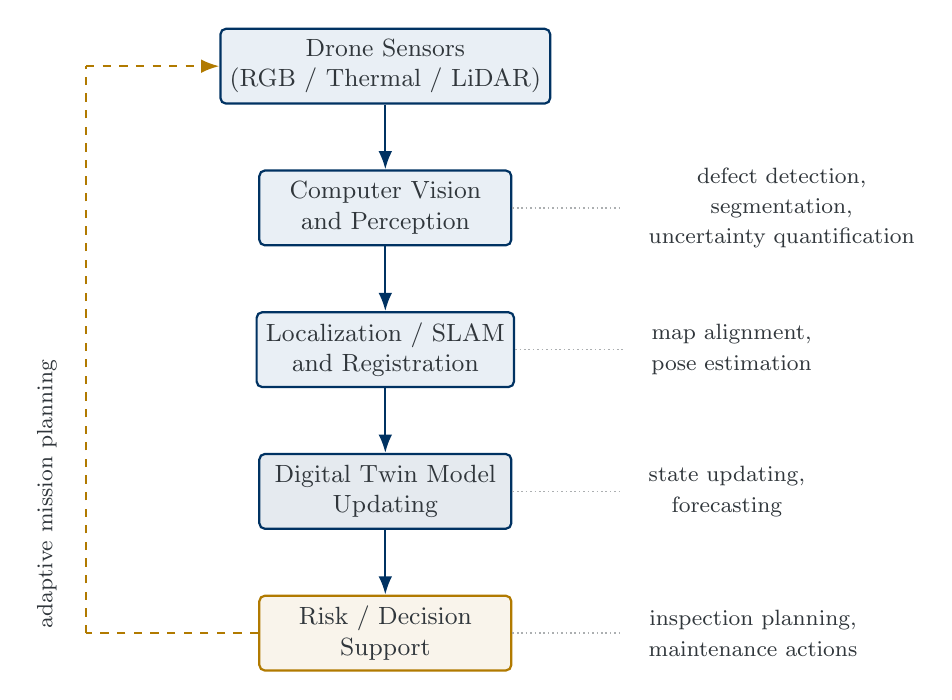
\begin{tikzpicture}[book figure,
    >=Latex,
    every node/.style={font=\small, align=center},
    block/.style={
        rectangle,
        rounded corners=2pt,
        draw,
        minimum width=3.2cm,
        minimum height=0.95cm,
        line width=0.8pt,
        fill=BookLight
    },
    arrow/.style={->, draw=BookBlue, line width=0.8pt},
    feedback/.style={->, draw=BookGold, dashed, line width=0.8pt}
]

% Main vertical workflow
\node[block] (sense) at (0,0) {Drone Sensors\\(RGB / Thermal / LiDAR)};
\node[block] (vision) at (0,-1.8) {Computer Vision\\and Perception};
\node[block] (slam) at (0,-3.6) {Localization / SLAM\\and Registration};
\node[block,fill=BookBlue!10] (dt) at (0,-5.4) {Digital Twin Model\\Updating};
\node[block,draw=BookGold,fill=BookGold!8] (risk) at (0,-7.2) {Risk / Decision\\Support};

\draw[arrow] (sense) -- (vision);
\draw[arrow] (vision) -- (slam);
\draw[arrow] (slam) -- (dt);
\draw[arrow] (dt) -- (risk);

% Side annotations
\node[right=1.6cm of vision] (ann1) {\footnotesize defect detection,\\\footnotesize segmentation, \\\footnotesize uncertainty quantification};
\node[right=1.6cm of slam]   (ann2) {\footnotesize map alignment,\\\footnotesize pose estimation};
\node[right=1.6cm of dt]     (ann3) {\footnotesize state updating,\\\footnotesize forecasting};
\node[right=1.6cm of risk]   (ann4) {\footnotesize inspection planning,\\\footnotesize maintenance actions};

% Optional connecting guide lines
\draw[BookInk!40,densely dotted,line width=0.6pt] (vision.east) -- ([xshift=-2mm]ann1.west);
\draw[BookInk!40,densely dotted,line width=0.6pt] (slam.east)   -- ([xshift=-2mm]ann2.west);
\draw[BookInk!40,densely dotted,line width=0.6pt] (dt.east)     -- ([xshift=-2mm]ann3.west);
\draw[BookInk!40,densely dotted,line width=0.6pt] (risk.east)   -- ([xshift=-2mm]ann4.west);

% Feedback loop: short horizontal out, vertical up, short horizontal in
\draw[dashed, draw=BookGold, line width=0.8pt]
(risk.west) -- (-3.8,-7.2);

\draw[dashed, draw=BookGold, line width=0.8pt]
(-3.8,-7.2) -- (-3.8,0);

\draw[feedback]
(-3.8,0) -- (sense.west);

% Vertical label parallel to dashed line
\node[rotate=90, font=\footnotesize, left=2mm]
at (-4.1,-3.6) {adaptive mission planning};

\end{tikzpicture}
\end{document}
